\documentclass{article}
\usepackage[paperwidth=8.8cm,paperheight=9.4cm,margin=0mm]{geometry}
\usepackage{graphicx}
\usepackage{xcolor}
\usepackage{tikz}
\pagestyle{empty}
\setlength{\parindent}{0pt}

\definecolor{panelbg}{HTML}{F8FAFC}
\definecolor{bordergray}{HTML}{CBD5E1}
\definecolor{darkgray}{HTML}{0F172A}
\definecolor{alertred}{HTML}{DC2626}
\definecolor{darkgreen}{HTML}{16A34A}

\begin{document}%
\begin{tikzpicture}[font=\sffamily]

% -------------------------------------------------------------
% ROW 1: CLINICAL ABDOMINAL CT
% -------------------------------------------------------------
\node[anchor=west, font=\fontsize{5.2pt}{6.2pt}\bfseries\selectfont, text=darkgray, inner sep=0pt] at (0.15, 9.15) 
    {Clinical Abdominal CT Volume (In Vivo Patient, $64^3$ ROI, 4 Chunks):};

% CT Before
\draw[draw=alertred, fill=black, rounded corners=1.5pt, line width=0.9pt] (0.15, 6.1) rectangle (2.85, 8.8);
\node[anchor=center] at (1.50, 7.45) {
\includegraphics[width=2.6cm, height=2.6cm]{ct_before.png}};
\node[anchor=north west, fill=alertred, text=white, font=\fontsize{4pt}{4.5pt}\bfseries\selectfont, rounded corners=1pt, inner sep=1pt] at (0.22, 8.73) {BEFORE};
% 4 lines below image
\node[anchor=north, align=center, text width=2.75cm, inner sep=0pt, font=\fontsize{3.8pt}{4.8pt}\selectfont, text=darkgray] at (1.50, 5.95) {
    \textbf{(a) Conventional Clip}\\
    Continuous + Rounding\\
    Phase Reset Error ($D_0$)\\
    92.2\% Error $\mid$ Streaks
};

% CT After
\draw[draw=darkgreen, fill=black, rounded corners=1.5pt, line width=0.9pt] (3.05, 6.1) rectangle (5.75, 8.8);
\node[anchor=center] at (4.40, 7.45) {
\includegraphics[width=2.6cm, height=2.6cm]{ct_after.png}};
\node[anchor=north west, fill=darkgreen, text=white, font=\fontsize{4pt}{4.5pt}\bfseries\selectfont, rounded corners=1pt, inner sep=1pt] at (3.12, 8.73) {AFTER};
% 4 lines below image
\node[anchor=north, align=center, text width=2.75cm, inner sep=0pt, font=\fontsize{3.8pt}{4.8pt}\selectfont, text=darkgray] at (4.40, 5.95) {
    \textbf{(b) AP-Bresenham}\\
    Exact Diophantine Entry\\
    Phase Injection $D(k)$\\
    0.0\% Error $\mid$ Bit-Exact
};

% CT Diff
\draw[draw=bordergray, fill=black, rounded corners=1.5pt, line width=0.7pt] (5.95, 6.1) rectangle (8.65, 8.8);
\node[anchor=center] at (7.30, 7.45) {
\includegraphics[width=2.6cm, height=2.6cm]{ct_diff.png}};
\node[anchor=north west, fill=black!75, text=white, font=\fontsize{4pt}{4.5pt}\bfseries\selectfont, rounded corners=1pt, inner sep=1pt] at (6.02, 8.73) {ERROR MAP};
% 4 lines below image
\node[anchor=north, align=center, text width=2.75cm, inner sep=0pt, font=\fontsize{3.8pt}{4.8pt}\selectfont, text=darkgray] at (7.30, 5.95) {
    \textbf{(c) Residual Error}\\
    Difference ($|\Delta I|$)\\
    Boundary Streak Noise\\
    Max Error = 15.94\,cm$^{-1}$
};


% -------------------------------------------------------------
% ROW 2: MNI-152 HUMAN BRAIN MRI
% -------------------------------------------------------------
\node[anchor=west, font=\fontsize{5.2pt}{6.2pt}\bfseries\selectfont, text=darkgray, inner sep=0pt] at (0.15, 4.45) 
    {MNI-152 Human Brain MRI Volume (Isotropic 1\,mm$^3$, 4 Chunks):};

% MRI Before
\draw[draw=alertred, fill=black, rounded corners=1.5pt, line width=0.9pt] (0.15, 1.40) rectangle (2.85, 4.10);
\node[anchor=center] at (1.50, 2.75) {
\includegraphics[width=2.6cm, height=2.6cm]{mri_before.png}};
\node[anchor=north west, fill=alertred, text=white, font=\fontsize{4pt}{4.5pt}\bfseries\selectfont, rounded corners=1pt, inner sep=1pt] at (0.22, 4.03) {BEFORE};
% 4 lines below image
\node[anchor=north, align=center, text width=2.75cm, inner sep=0pt, font=\fontsize{3.8pt}{4.8pt}\selectfont, text=darkgray] at (1.50, 1.25) {
    \textbf{(d) Conventional Clip}\\
    Continuous + Rounding\\
    Phase-Shift Seam Jump\\
    90.2\% Error $\mid$ Step Shift
};

% MRI After
\draw[draw=darkgreen, fill=black, rounded corners=1.5pt, line width=0.9pt] (3.05, 1.40) rectangle (5.75, 4.10);
\node[anchor=center] at (4.40, 2.75) {
\includegraphics[width=2.6cm, height=2.6cm]{mri_after.png}};
\node[anchor=north west, fill=darkgreen, text=white, font=\fontsize{4pt}{4.5pt}\bfseries\selectfont, rounded corners=1pt, inner sep=1pt] at (3.12, 4.03) {AFTER};
% 4 lines below image
\node[anchor=north, align=center, text width=2.75cm, inner sep=0pt, font=\fontsize{3.8pt}{4.8pt}\selectfont, text=darkgray] at (4.40, 1.25) {
    \textbf{(e) AP-Bresenham}\\
    Exact Diophantine Entry\\
    Phase Injection $D(k)$\\
    0.0\% Error $\mid$ Seamless
};

% MRI Diff
\draw[draw=bordergray, fill=black, rounded corners=1.5pt, line width=0.7pt] (5.95, 1.40) rectangle (8.65, 4.10);
\node[anchor=center] at (7.30, 2.75) {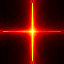
\includegraphics[width=2.6cm, height=2.6cm]{mri_diff.png}};
\node[anchor=north west, fill=black!75, text=white, font=\fontsize{4pt}{4.5pt}\bfseries\selectfont, rounded corners=1pt, inner sep=1pt] at (6.02, 4.03) {ERROR MAP};
% 4 lines below image
\node[anchor=north, align=center, text width=2.75cm, inner sep=0pt, font=\fontsize{3.8pt}{4.8pt}\selectfont, text=darkgray] at (7.30, 1.25) {
    \textbf{(f) Residual Error}\\
    Difference ($|\Delta I|$)\\
    Boundary Step Error\\
    Max Signal Diff = 41.61
};

\end{tikzpicture}%
\end{document}
